\section{Wednesday for MAT4002}\index{Monday_lecture}
\subsection{Applications on the isomorphism of fundamental group}

\begin{theorem}
\[
\pi_1(S^1)\cong(\mathbb{Z},+)
\]
\end{theorem}
\begin{proof}
Define the orientation of $|K|$ as shown in Fig.~(\ref{fig:13:8}).
\begin{figure}[H]
\centering
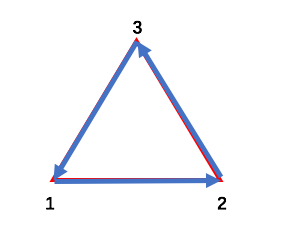
\includegraphics[width=0.3\textwidth]{week13/f_30}
\caption{Orientation of $|K|$
} 
\label{fig:13:8}
\end{figure}
Following the proof during last lecture, we construct 
\[
\begin{array}{ll}\phi:
&E(K,1)\to (\mathbb{Z},+)\\\text{with}&[\alpha]\mapsto
\text{winding number of $\alpha$}
\end{array}
\]
where the winding number of $\alpha$ is the 
\[
\text{number of 23 appearing in $\alpha$} - \text{number of 32 appearing in $\alpha$}.
\]

Note that
\begin{enumerate}
\item
The winding number is invariant under elementary contraction and elementary expansion.
\item
In particular,
\begin{align*}
\text{winding number for }(1\underbrace{23\cdots123}_{23 \text{ shows for $m$ times}}1)&=m\\
\text{winding number for }(1\underbrace{32\cdots132}_{32 \text{ shows for $n$ times}}1)&=-n\\
\end{align*}
\item
For any given $\alpha$, it is equivalent to a unique $(123123\cdots1231)$ or $(132\cdots1321)$, since otherwise $\alpha$ will have different winding numbers.
\end{enumerate}
Therefore, (1) and (3) shows the well-definedness of $\phi$. In particular, $(1)$ shows that as $\alpha\sim\alpha'$, we have $\phi([\alpha])=\phi([\alpha'])$; $(2)$ shows that the winding number of $\alpha$ is an unique integer.
\begin{itemize}
\item
Homomorphism:
For given any two edge loops $\alpha,\beta$ based at $1$, suppose that $[\alpha]=[(1bc1bc\cdots1bc1)]$ and $[\beta]=[(1pq1pq\cdots1pq1)]$, then
\[
\phi([\alpha]\cdot[\beta])=\phi([\alpha\cdot\beta])
=
[(1bc1bc\cdots1bc11pq1pq\cdots1pq1)]
\]
Discuss the case for the sign of $\phi([\alpha])$ and $\phi([\beta])$ separately gives the desired result.
\item
Surjectivity:
for a given $m\in\mathbb{Z}$,
construct $\alpha$ such that $\phi([\alpha])=m$ is easy.
\item
Injectivity:
suppose that $\phi([\alpha])=0$, then by definition of $\phi$, $[\alpha]=[(1)]=e$, which is the trivial element in $E(K,1)$.
\end{itemize}
Therefore, $\phi$ is an isomorphism.
\end{proof}

\begin{remark}
Actually, we can show that the loop based at $1$ given by:
\[
\begin{array}{ll}
\ell&I\to S^1\\\text{with}&t\mapsto e^{2\pi i t}
\end{array}
\]
is a generator for $\pi_1(S^1,1)$:
\begin{itemize}
\item
$\phi([\ell])=1$, where $\phi:\pi_1(S^1,1)\cong\mathbb{Z}$.
\item
The loop
\[
\begin{array}{ll}
\ell^m:&I\to S^1\quad m\in\mathbb{Z}\\
\text{with}&\ell^m(t) = e^{2\pi imt}
\end{array}
\]
gives $\phi([\ell^m])=m$
\end{itemize}
\end{remark}

\begin{corollary}[Fundamental Theorem of Algebra]
All non-constant polynomials in $\mathbb{C}$ has at least one root in $\mathbb{C}$
\end{corollary}

\begin{proof}
\begin{itemize}
\item
Suppose on the contrary that 
\[
p(x)=a_nx^n+\cdots+a_1x+a_0\ a_n\ne0
\]
has no roots, then $p$ is a mapping from $\mathbb{C}$ to $\mathbb{C}\setminus\{0\}$.
It's clear that $\mathbb{C}\setminus\{0\}\simeq\{z\in\mathbb{C}\mid|z|=1\}$, and therefore
\[
\pi_1(\mathbb{C}\setminus\{0\})=\pi_1(S^1)\cong\mathbb{Z}.
\]
\item
The induced homomorphism $p^*$ of $p$ is given by:
\[
\begin{array}{ll}
p_*:&\pi_1(\mathbb{C})\to \pi_1(\mathbb{C}\setminus\{0\})\\
\text{with}&\{e\}\mapsto\mathbb{Z}
\end{array}
\]
Note that $\pi_1(\mathbb{C})$ is trival as $\mathbb{C}$ is contractible. Also, $p_*(e)=0$.
\item
Consider the inclusion from $C_r=\{z\in\mathbb{C}\mid |z|=r\}$ to $\mathbb{C}$:
\[
\begin{array}{ll}
i:&C_r\to\mathbb{C}\\
\text{with}&z\mapsto z
\end{array}
\]
It satisfies the diagram given below:
\begin{figure}[H]
\centering
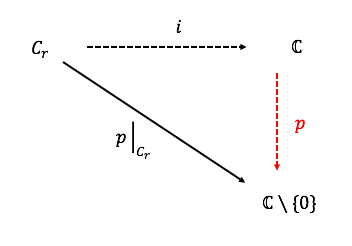
\includegraphics[width=0.5\textwidth]{week13/f_31}
\end{figure}
As a result, the induced homomorphism $i^*$ of $i$ satisfies the diagram
\begin{figure}[H]
\centering
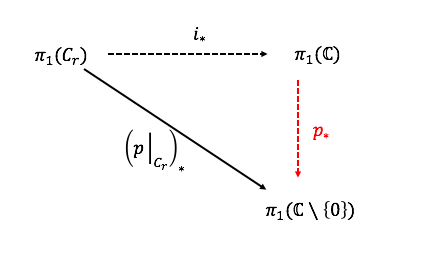
\includegraphics[width=0.5\textwidth]{week13/f_32}
\end{figure}
Or equivalently,
\begin{figure}[H]
\centering
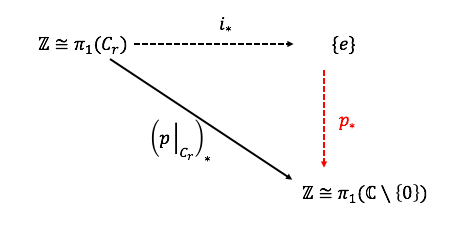
\includegraphics[width=0.5\textwidth]{week13/f_33}
\end{figure}
Therefore, $p_*\circ i_*$ is a zero map since $p_*(e)=0$, i.e., $(p\mid_{C_r})_*$ is a zero homomorphism.
\item
Then it's natural to study $p\mid_{C_r}:C_r\to\mathbb{C}\setminus\{0\}$.
Construct 
\[
\left\{
\begin{aligned}
q(z)&=k\cdot z^n,\quad k:=\frac{p(r)}{r^n}\text{is a constant}\\
p(z)&=a_nz^n+\cdots+a_1z+a_0
\end{aligned}
\right.
\]
Therefore, $p(r)=q(r)$, and $p|_{C_r},q|_{C_r}:C_r\to\mathbb{C}\setminus\{0\}$.
\begin{itemize}
\item
We claim that $p|_{C_r}\simeq q|_{C_r}$ for large $r$.
First construct the mapping 
\[
\begin{array}{ll}
H:&C_r\times[0,1]\to\mathbb{C}\\
\text{with}&H(z,t)=tp(z)+(1-t)q(z)\\
\text{and}&H(z,0)=q(z), \ H(z,1) = p(z)\\
\end{array}
\]
If we want to show $H$ is the homotopy between $p|_{C_r}$ and $q|_{C_r}$, it suffices to show that $H$ is well-defined, i.e., $H:c_r\times[0,1]\to\mathbb{C}\setminus\{0\}$.

Suppose on the contrary that there exists $(z,t)$ such that
\[
(1-t)p(z)+tq(z)=0,\quad |z|=r, t\in[0,1]
\]
Or equivalently,
\[
(1-t)(a_nz^n+\cdots+a_1z+a_0)+t\cdot kz^n=0.
\]
Substituting $k$ with $p(r)/r^n$ gives 
\[
a_nz^n+\cdots+a_1z+a_0
=
t\left(
a_{n-1}z^{n-1}+\cdots+a_0 - a_{n-1}\frac{z^n}{r}-\cdots-a_1\frac{z^n}{r^{n-1}}-a_0\frac{z^n}{r^n}
\right)
\]
The LHS has leading order $n$, while the RHS has leading order less or equal to $n-1$.
As $r=|z|\to\infty$, $t\to\infty$. Therefore, the equality does not hold in the range $t\in[0,1]$ when $r$ is sufficiently large.

For this choice of $r=|z|$, 
\[
H:c_r\times[0,1]\to\mathbb{C}\setminus\{0\}
\]
gives the homotopy $p|_{C_r}\simeq q|_{C_r}$.
\end{itemize}
\item
Therefore, we imply $(p|_{C_r})_*=(q|_{C_r})_*$.
Now we check the mapping $(q|_{C_r})_*:\mathbb{Z}\to\mathbb{Z}$.
In particular, we check the value of $(q|_{C_r})_*(e)$, where $e$ is the identity in $\pi_1(C_r)$.
Here we construct the loop
\[
\begin{array}{ll}
\ell:&I\to C_r\\
\text{with}&\ell(t)=re^{2\pi it}
\end{array}
\]
and therefore $[\ell]=e$. It follows that 
\[
(q|_{C_r})_*(e) = (q|_{C_r})_*([\ell])=[q|_{C_r}(\ell)]=q(re^{2\pi it})=k\cot r^n\cdot e^{2\pi int}\ne0.
\]
Therefore, $(q|_{C_r})_*$ is not a zero homomorphism, i.e., $(p|_{C_r})_*\cong (q|_{C_r})_*$ is not a zero homomorphism, which is a contradiction.
\end{itemize}

\end{proof}













